\documentclass[12pt]{article}


\def\pdfpsfrag{no}
\def\reusepsfragpdf{yes or no}
\def\foiltex{no}
\def\algfontmode{no}
\input{../../FrequentlyUsed/latex/mydefs}

\usepackage{fullpage}
\usepackage{tikz}
\usetikzlibrary{decorations.pathreplacing}

\title{Kinetic dynamics}
\author{Sunghee Yun - Beth's Daddy \& Liam, Lucy, Adrian \& Lillian's Uncle}

\begin{document}
\maketitle
\tableofcontents

\section{Force equations}

\subsection{Ideal springs}

Suppose (simple) rules for springs hold. That is when a spring with $k\in\ppreals$ as the spring constant and $l\in\ppreals$ as the natural length
and two point masses $m_1\in\ppreals$ and $m_2\in\ppreals$, which are located at
$x_1\in\reals^3$
and
$x_2\in\reals^3$
as show in \figurename~\ref{fig:spring}.
The force exerted on $m_1$ is
\begin{equation}
\label{eq:force:spring}
	F_s(x_1;k,l,x_2) = -k (\|x_1-x_2\| - l) v_{2,1}
	= -k \left(\frac{\|x_1-x_2\| - l}{\|x_1-x_2\|}\right) (x_1-x_2)
\end{equation}
where $v_{2,1}\in\reals^3$ is a length-one vector pointing to the direction of $x_1$ from view point of $x_2$.
The force exerted on $m_2$ $F_s(x_2;k,l,x_1)$ be can obtained using 

\begin{figure}
\begin{center}
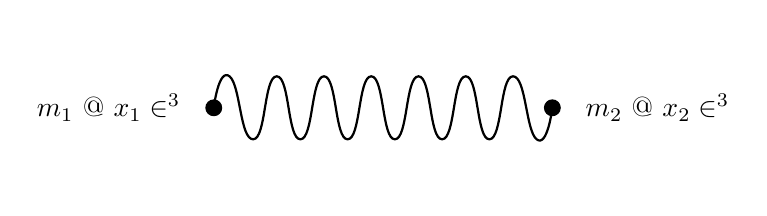
\begin{tikzpicture}[scale=1]
\def\coils{6} % Number of coils
\def\radius{0.4} % Radius of coils
\def\length{5} % Total length of spring
\def\startx{-2} % Starting x coordinate
\def\starty{0} % Starting y coordinate
\def\slope{2} % Height increase over length

%    \draw[very thin, dashed] (-3.5, -1) rectangle (3.8, 1); % Rectangle boundary
	\node[inner sep=0pt, outer sep=0pt] (left) at (-3.5, 0) {};
    \node[inner sep=0pt, outer sep=0pt] (right) at (3.8, 0) {};
    \node[inner sep=0pt, outer sep=0pt] (top) at (0, 1) {};
    \node[inner sep=0pt, outer sep=0pt] (bottom) at (0, -1) {};
    % Draw balls

	\def\ballo{(-2, 0)}
    \def\ballt{(2.3, 0)}
    
    % Draw balls
    \draw[fill=black] \ballo circle (0.1); % Ball 1
    \draw[fill=black] \ballt circle (0.1); % Ball 2

	\node[left=.3cm] at (-2, 0) {$m_1$ @ $x_1\in\reals^3$};
    \node[right=.3cm] at (2.3, 0) {$m_2$ @ $x_2\in\reals^3$};

\draw[thick] plot[smooth, tension=1]
  coordinates {
    (\startx+0.0,\starty)
    (\startx+0.2,\starty+\radius)
    (\startx+0.5,\starty-\radius)
    (\startx+0.8,\starty+\radius)
    (\startx+1.1,\starty-\radius)
    (\startx+1.4,\starty+\radius)
    (\startx+1.7,\starty-\radius)
    (\startx+2.0,\starty+\radius)
    (\startx+2.3,\starty-\radius)
    (\startx+2.6,\starty+\radius)
    (\startx+2.9,\starty-\radius)
    (\startx+3.2,\starty+\radius)
    (\startx+3.5,\starty-\radius)
    (\startx+3.8,\starty+\radius)
    (\startx+4.1,\starty-\radius)
    (\startx+4.3,\starty)
  };
\end{tikzpicture}
\end{center}
\caption{A spring connecting two point masses}
\label{fig:spring}
\end{figure}

\subsection{Gravity-like forces}

In a real world we live, we feel the gravity dragging us downward.
But since we can assume anything here! :)
let us assume that there exists gravity-like force
in a sense that given an acceleration vector $a\in\reals^3$,
the force exerted on a point mass $m\in\ppreals$ located at $x\in\reals^3$
is
\begin{equation}
\label{eq:force:gravity-like}
F_g(m;a) = ma
	\in\reals^3
\end{equation}
\ie,
the magnitude of the force is proportional to $m$ (and the magnitude of the acceleration),
the direction is the same as that of the acceleration.
It does \emph{not} depend on the location.

A typical example, of course, is \emph{the} gravity where
\[
	a = g = (0,0,-g)
	\in\reals^3
\]
where $g = 9.8 m/s^2$.

\subsection{Frictional forces}

We model frictional forces exerted on bodies (not point mass)
using the coefficient of friction $c\in\ppreals$ where the force is modeled by

\begin{equation}
\label{eq:force:frictional}
F_f(v) = -c v
	\in\reals^3
\end{equation}
where $v\in\reals^3$ is the velocity along the surface.

\section{Energies}

\subsection{Kinetic energy of a mass}

The kinetic energy of a mass $m$ with velocity $v\in\reals^3$
is defined by
\begin{equation}
\label{eq:energy:kinetic}
	E_\mathrm{k}(m) = \frac{1}{2} m\|v\|^2
\end{equation}

\subsection{Potential energy}

Note that the role of the potential energies in dynamics
is played in a way that the difference of them at two location,
hence adding a constant to any potential energy
makes no difference.

\subsubsection{Potential energy by a gravity-like force}

The potential energy of a mass $m$ by a gravity-like force with acceleration $a\in\reals^3$
is defined by
\begin{equation}
\label{eq:energy:potential:gravity-like}
E_\mathrm{p,g}(m,x;a)
=  - m x\cdot a
= - m x^Ta
\end{equation}
where $a^Tb = a\cdot b$ for two vectors $a$ and $b$
is the inner product.
For example, the potential energy by gravity is
\[
	E_\mathrm{p,g}(m,x;g)
	=  mgx_3
\]

\subsubsection{Potential energy by a spring}

The potential energy of a mass $m$ by a gravity-like force with acceleration $a\in\reals^3$
is defined by
\begin{equation}
\label{eq:energy:potential:spring}
E_\mathrm{p,s}(x_1,x_2;k,l)
= \frac{k}{2} (\|x_1-x_2\|-l)^2
\end{equation}


\subsection{The law of preservation of the energy}

In a system with masses, springs, and gravity-like forces with no frictional forces,
the sum of the kinetic energies of all the masses
and that of the potential energies of all the gravity-like forces and springs
is preserved
unless, for example, external forces are exerted on the system,
two point masses merge into one,
or some non-elastic crashes happen.

\subsubsection{Proof}

XXX

\subsection{Dissipated energy by a frictional force}

The energy dissipated due to a frictional force exerted on a mass
can be calculated by
\begin{equation}
\int F_f(v) \cdot dx
\end{equation}

\subsection{The law of preservation of the energy with frictional forces}

In a system with masses, springs, and gravity-like forces \emph{with} frictional forces,
the sum of the kinetic energies and potential energies is reduced
and the amount of reduction is (exactly) the same as the total dissipated energy.


\section{Momentum}

The momentum of a mass $m$ with velocity $v$ is defined by
\begin{equation}
M(m,v) = mv \in\reals^3
\end{equation}

\subsection{The law of preservation of the momentum}

In a system with masses,
the sum of all the momentum of all the masses
is preserved
unless, for example, external forces are exerted on the system
even when, for example, two point masses merge into one or some non-elastic crashes happen.


\subsubsection{Proof}

XXX

\section{Equilibrium point}

An equilibrium point of a system
is defined by the configuration of all the masses in the system
so as to minimize the total energy
or equivalently, 
that where the force exerted on every mass, \ie, the sum of all the forces exerted on every mass,
is zero.


\subsection{Finding the equilibrium point}

\end{document}
